%\newpage
%\section{Metodologia Experimental}
%
%\subsection{Materiais}
%
%Para a realização do experimento foi utilizado o software Simulink do pacote Matlab.
%
%O experimento foi realizado em três partes. De início, foi estudado o comportamento da modulação ASK multinível. Em seguida, foi analisada a modulação FSK multinível e por ultimo, a modulação PSK multinível.
%
%\subsection{Simulação M-ASK}
%Na primeira atividade, foi montado o circuito da figura \ref{fig:ASK} com ajuda do roteiro que continha todos os parâmetros necessários para configurar os blocos.
%
%\begin{figure}[H]
%    \centering
%    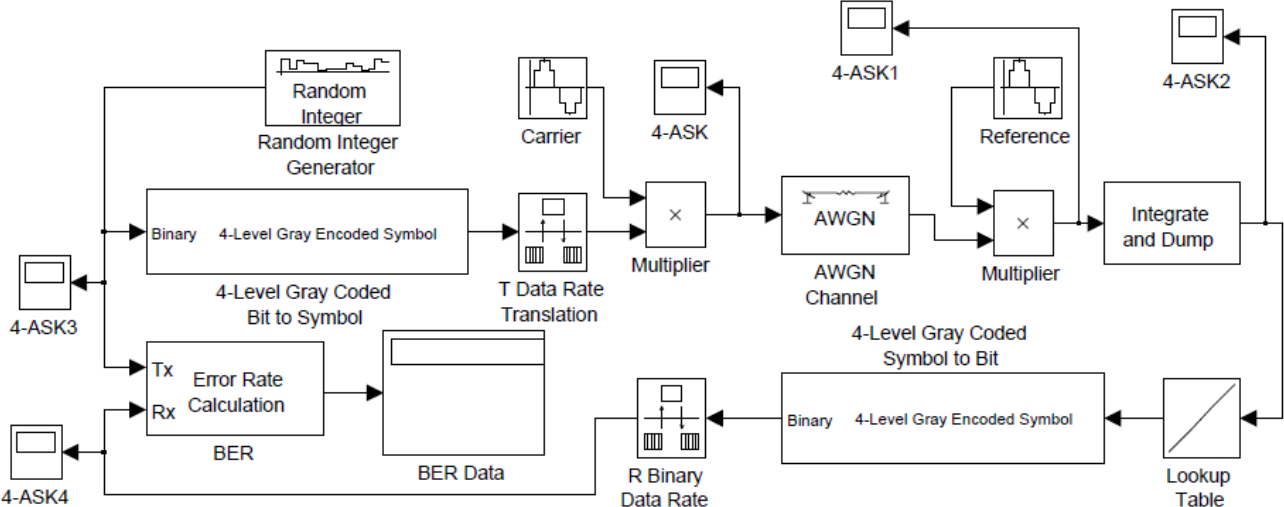
\includegraphics[scale=0.3]{ASK}
%    \caption{Diagrama do sistema 4-ASK.}
%    \label{fig:ASK}
%\end{figure}
%
%Um sistema de comunicação digital ASK retangular 4-ário com canal AWGN e um receptor coerente ótimo implementado com um integrador e um limiar é mostrado na figura \ref{fig:ASK}. Os pulsos 4-ASK retangular tem, a priori, igual probabilidade de ocorrência.
%O sistema de comunicação 4-ASK retangular com código Gray de 2 bits é similar ao sistema retangular não codificado. O código Gray atribuí entrada de i-bits 00, 01, 10 e 11 como os quatro níveis de saída 0, 1, 3 e 2, respectivamente.Os parâmetros de simulação devem ser ajustados de acordo com o roteiro.
%
%O próximo passo é montar um codificador para código \textit{Gray}, conforme a figura \ref{fig:GrayEncoder}.
%Para recuperar a informação, é necessário montar um conversor símbolos \textit{Gray} para pulsos binários, conforme a figura \ref{fig:GrayDecoder}.
%
%\begin{figure}[H]
%    \centering
%    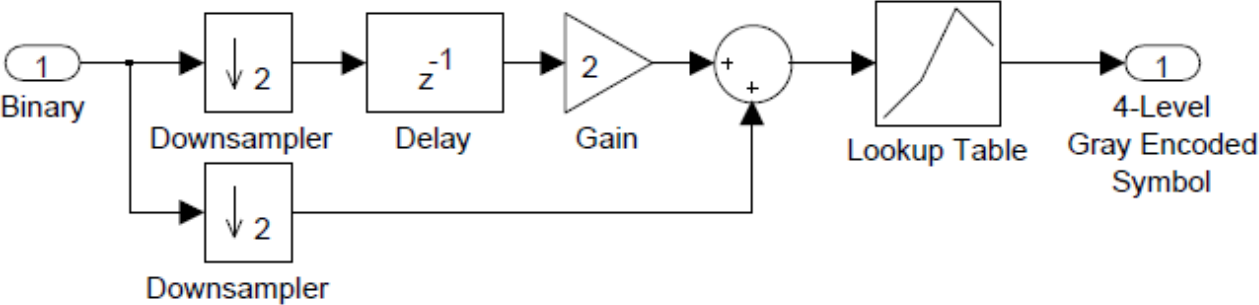
\includegraphics[scale=0.3]{GrayEncoder}
%    \caption{Conversor de binário para código \textit{Gray}.}
%    \label{fig:GrayEncoder}
%\end{figure}
%
%\begin{figure}[H]
%    \centering
%    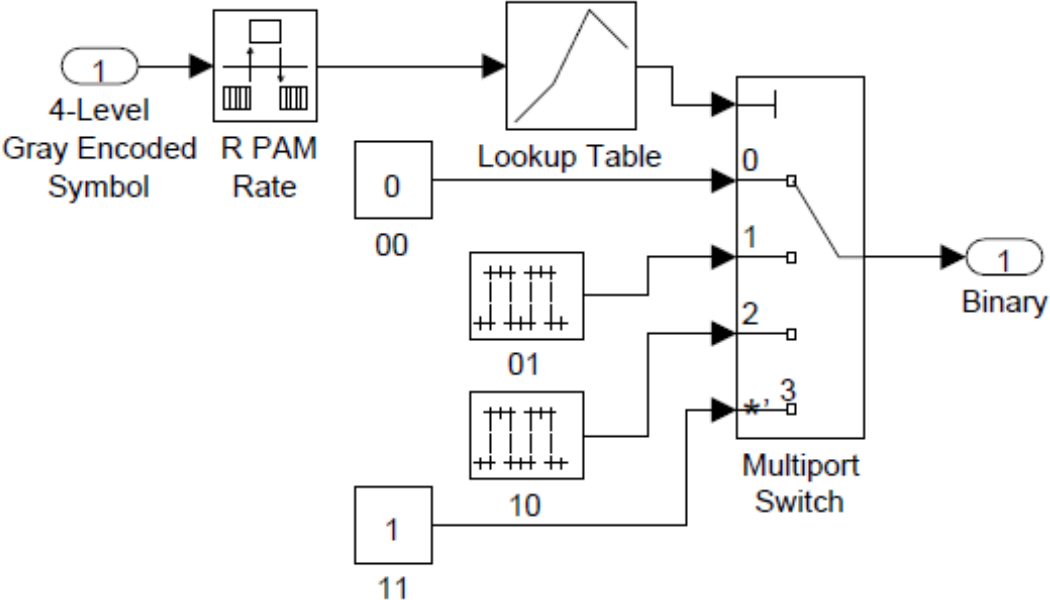
\includegraphics[scale=0.4]{GrayDecoder}
%    \caption{Conversor de símbolos em codificação \textit{Gray} para binário.}
%    \label{fig:GrayDecoder}
%\end{figure}
%
%Em seguida, obter os gráficos nos pontos onde há osciloscópio  para o 4-ASK e também verificar o atraso no sinal recebido em relação ao transmitido. Plotar o gráfico BER x Eb/No (semilogy). 
%
%Em seguida, montar uma tabela de acordo com a tabela \ref{tab:1}, com os dados obtidos nas simulações. O valor de $P_b$ é dado pela equação \ref{eq:pbask}.
%
%\begin{equation}
%\label{eq:pbask}
%P_{b,4 bits, cod. Gray} = \frac{3}{4}\mathcal{Q}\left(\sqrt{\frac{0,286E_b}{N_0}} \right)
%\end{equation}
%
%Como ultimo passo, obter o gráfico da densidade espectral de potência (PSD) da modulação 4-ASK com os blocos mostrados na figura \ref{fig:PSD-ASK}.
%
%\begin{figure}[H]
%    \centering
%    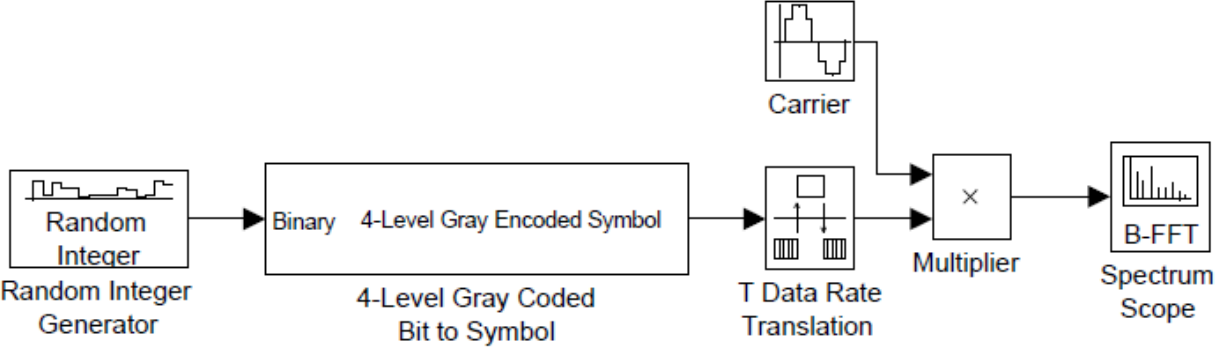
\includegraphics[scale=0.35]{PSD-ASK}
%    \caption{Blocos para obtenção do gráfico da PSD da modulação 4-ASK utilizada.}
%    \label{fig:PSD-ASK}
%\end{figure}
%
%\begin{small}
%    \begin{table}[H]
%        \begin{center}
%            \caption{Tabela BER x Eb/No para modulação 4-ASK}
%            \begin{tabular}{c|c|c}
%                \hline
%                $\frac{Eb}{No}$ [dB] & BER & $P_b$ \\
%                \hline
%                14 & $2,3 \times 10^{-3} $ & \\
%                \hline
%                12 & & $1,27 \times 10^{-2} $\\
%                \hline
%                10 & & \\
%                \hline
%                8 & & \\
%                \hline
%                6 & & \\
%                \hline
%                4 & & \\
%                \hline
%                2 & & \\
%                \hline
%                0 & & \\
%                \hline
%            \end{tabular}
%            \label{tab:1}
%        \end{center}
%    \end{table}
%\end{small}
%
%
%\subsection{Modulação M-FSK}
%Como próxima atividade, simular o circuito 4-FSK com codificação binária.
%
%\begin{figure}[H]
%    \centering
%    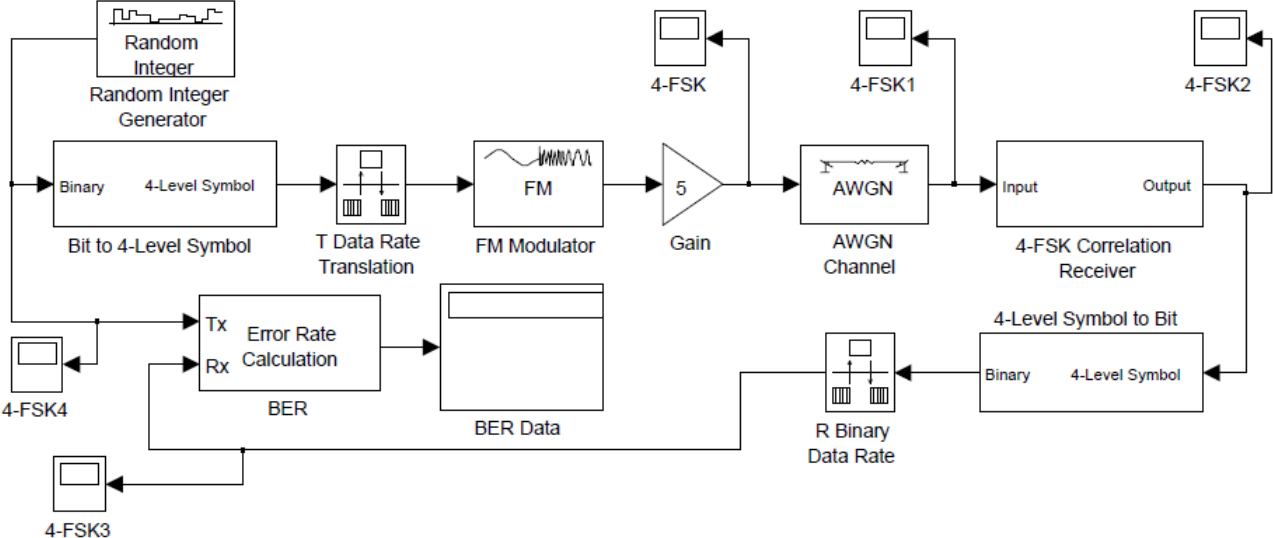
\includegraphics[scale=0.3]{FSK}
%    \caption{Sistema 4-FSK com codificação binária.}
%    \label{fig:FSK}
%\end{figure}
%
%Os blocos com o codificador e decodificador binário estão nas figuras \ref{fig:BinEncoder} e \ref{fig:BinDecoder}, respectivamente.
%
%\begin{figure}[H]
%    \centering
%    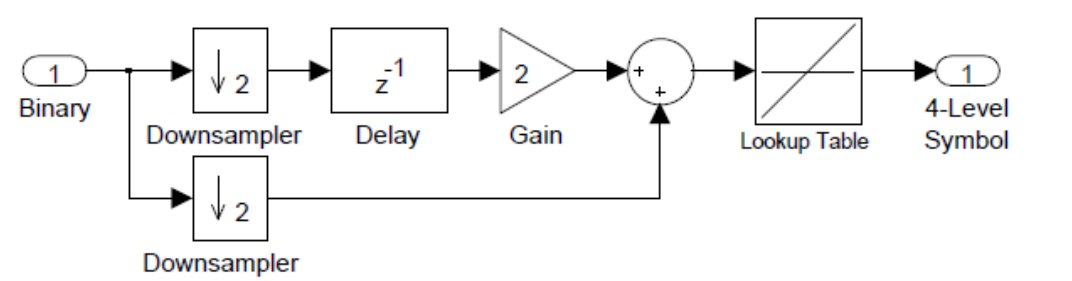
\includegraphics[scale=0.35]{BinEncoder}
%    \caption{Blocos para codificação em binário.}
%    \label{fig:BinEncoder}
%\end{figure}
%
%\begin{figure}[H]
%    \centering
%    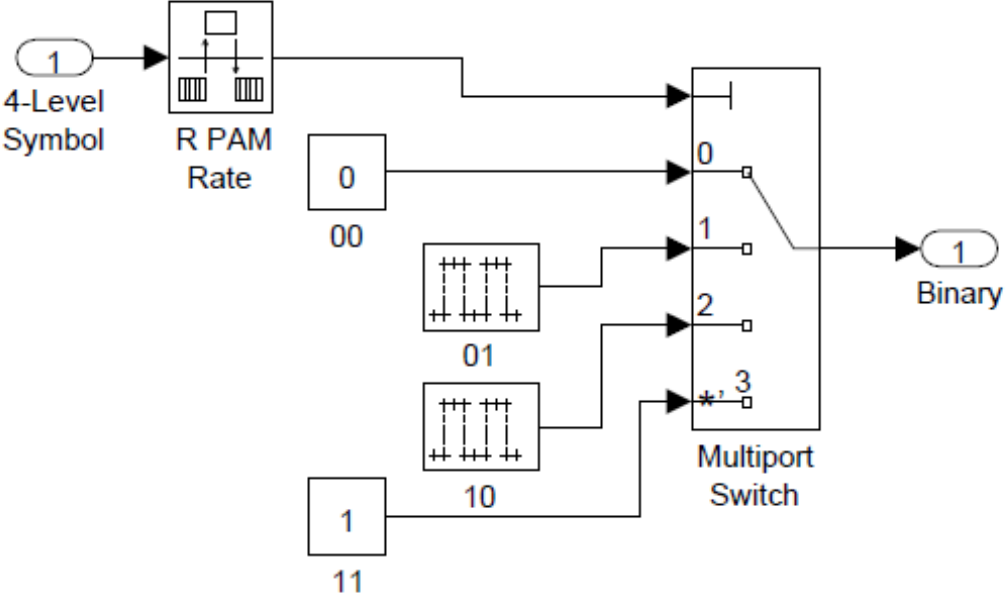
\includegraphics[scale=0.35]{BinDecoder}
%    \caption{Blocos para decodificação de binário.}
%    \label{fig:BinDecoder}
%\end{figure}
%
%Por conseguinte, gerar os gráficos nos pontos onde possui o osciloscópio. Verificar o atraso no sinal recebido em relação ao transmitido e plotar o gráfico BER x Eb/No (semilogy). A tabela \ref{tab:2} deverá ser preenchida com os dados encontrados.
%A equação \ref{eq:pbfsk} deve ser utilizada para encontrar os valores de $P_b$.
%
%
%\begin{equation}
%\label{eq:pbfsk}
%P_{b,4 bits, cod. binária} = \frac{M}{2}\mathcal{Q}\left(\sqrt{\log_2 M \left[\frac{E_b}{N_0}\right]} \right) \qquad para \, M > 4.
%\end{equation}
%
%
%\begin{small}
%    \begin{table}[H]
%        \begin{center}
%            \caption{Tabela BER x Eb/No para 4-FSK com codificação binária.}
%            \begin{tabular}{c|c|c}
%                \hline
%                $\frac{Eb}{No}$ [dB] & BER & $P_b$ \\
%                \hline
%                8 & $1 \times 10^{-4}$ & \\
%                \hline
%                6 & & $4,8 \times 10^{-3}$ \\
%                \hline
%                4 & & \\
%                \hline
%                2 & & \\
%                \hline
%                0 & & \\
%                \hline
%            \end{tabular}
%            \label{tab:2}
%        \end{center}
%    \end{table}
%\end{small}
%
%Obter também o gráfico da densidade espectral de potência com os blocos da figura \ref{fig:PSD-FSK}.
%
%\begin{figure}[H]
%    \centering
%    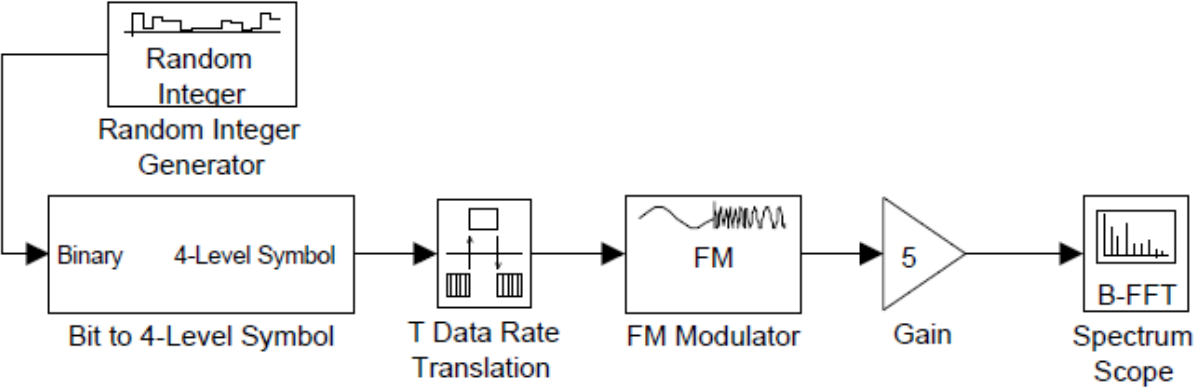
\includegraphics[scale=0.3]{PSD-FSK}
%    \caption{Blocos para obter a PSD para modulação FSK.}
%    \label{fig:PSD-FSK}
%\end{figure}
%
%\subsection{Modulação M-PSK}
%Como próxima atividade, simular o circuito 4-PSK com codificação \textit{Gray}.
%
%\begin{figure}[H]
%    \centering
%    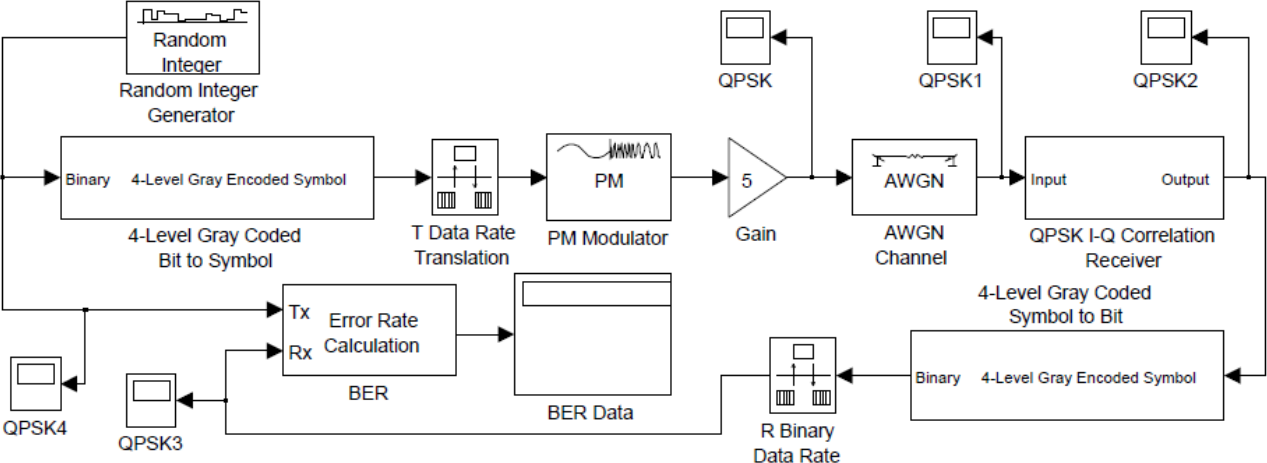
\includegraphics[scale=0.3]{PSK}
%    \caption{Sistema 4-PSK com codificação \textit{Gray}.}
%    \label{fig:PSK}
%\end{figure}
%
%Os blocos com o codificador e decodificador binário estão nas figuras \ref{fig:GrayEncoder} e \ref{fig:GrayDecoder}, respectivamente.
%
%Gerar os gráficos nos pontos onde possui o osciloscópio. Verificar o atraso no sinal recebido em relação ao transmitido e plotar o gráfico BER x Eb/No (semilogy). A tabela \ref{tab:3} deverá ser preenchida com os dados encontrados.
%A equação \ref{eq:pbpsk} deve ser utilizada para encontrar os valores de $P_b$.
%
%
%\begin{equation}
%\label{eq:pbfsk}
%P_{b,4 bits, cod. Gray} = \frac{M}{M-1}\mathcal{Q}\left(\sqrt{2 \log_2 M \left[\frac{E_b}{N_0}\right]sen^2\frac{\pi}{M}} \right) \qquad para \, M > 4.
%\end{equation}
%
%
%\begin{small}
%    \begin{table}[H]
%        \begin{center}
%            \caption{Tabela BER x Eb/No para 4-PSK com codificação \textit{Gray}.}
%            \begin{tabular}{c|c|c}
%                \hline
%                $\frac{Eb}{No}$ [dB] & BER & $P_b$ \\
%                \hline
%                8 & $2 \times 10^{-4}$ & \\
%                \hline
%                6 & & $2,4 \times 10^{-3}$ \\
%                \hline
%                4 & & \\
%                \hline
%                2 & & \\
%                \hline
%                0 & & \\
%                \hline
%            \end{tabular}
%            \label{tab:3}
%        \end{center}
%    \end{table}
%\end{small}
%
%Obter também o gráfico da densidade espectral de potência com os blocos da figura \ref{fig:PSD-PSK}.
%
%\begin{figure}[H]
%    \centering
%    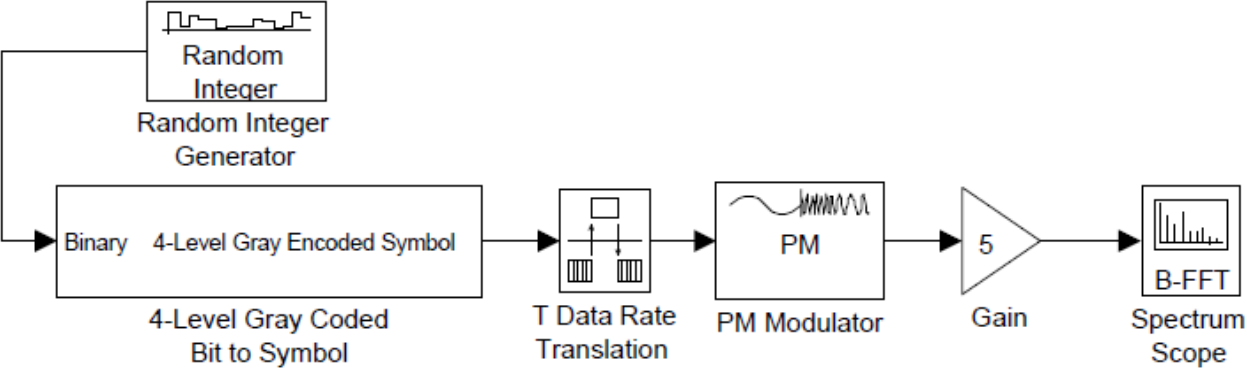
\includegraphics[scale=0.3]{PSD-PSK}
%    \caption{Blocos para obter a PSD para modulação PSK.}
%    \label{fig:PSD-PSK}
%\end{figure}
%
%\subsection{Comparação entre as técnicas de modulação}
%
%Como ultimo passo, montar um gráfico contendo a BER para os três tipo de modulação estudados e comparar o desempenho das mesmas.